%%%%%%%%%%%%%%%%%%%%%%%%%%%%%%%%%%%%%%%%%%%%%%%%%%%%%%%%%%%%%%%%%%%%%%%%%%%%
% Step 1: Set the \documentclass
%% To submit your paper:
\documentclass[draft]{agujournal2019}
\usepackage{url} %this package should fix any errors with URLs in refs.
\usepackage{lineno}
\usepackage[inline]{trackchanges} %for better track changes. finalnew option will compile document with changes incorporated.
\usepackage{soul}
\usepackage{float}
\usepackage{listings}
\linenumbers
\usepackage{minted}
\usepackage{xcolor} % to access the named colour LightGray
\usepackage{url}

%% Choose from this list of Journals:
% JGR: Atmospheres
% JGR: Biogeosciences
% JGR: Earth Surface
% JGR: Oceans
% JGR: Planets
% JGR: Solid Earth
% JGR: Space Physics
% Global Biogeochemical Cycles
% Geophysical Research Letters
% Paleoceanography and Paleoclimatology
% Radio Science
% Reviews of Geophysics
% Tectonics
% Space Weather
% Water Resources Research
% Geochemistry, Geophysics, Geosystems
% Journal of Advances in Modeling Earth Systems (JAMES)
% Earth's Future
% Earth and Space Science
% Geohealth
\journalname{Space Weather}


\begin{document}

%% ------------------------------------------------------------------------ 
%  Title
%% ------------------------------------------------------------------------ 
\title{PyIRI: Whole-Globe Approach to the International Reference Ionosphere Modeling Implemented in Python}

%% ------------------------------------------------------------------------ 
%  AUTHORS AND AFFILIATIONS
%% ------------------------------------------------------------------------ 

\authors{Victoriya V. Forsythe\affil{1}, Dieter Bilitza\affil{1,2},  Angeline Burrell\affil{1}, Douglas P. Drob\affil{1}, Kenneth Dymond\affil{1}, Bruce Fritz\affil{1}, Sarah McDonald\affil{1}}

\affiliation{1}{U.S. Naval Research Laboratory, Washington, DC, USA}
\affiliation{2}{Department of Physics and Astronomy, George Mason University, Fairfax, VA, USA}
\affiliation{3}{Heliospheric Laboratory, NASA
Goddard Space Flight Center, Greenbelt, MD, USA}


\correspondingauthor{Victoriya V. Forsythe}{victoriya.makarevich@nrl.navy.mil}


\begin{keypoints}
\item Python tool for rapid global ionospheric electron density estimates
\item Novel approach to CCIR coefficients and IRI model
\item 24-hour global electron density in a few seconds 
\end{keypoints}


\begin{abstract}
International Reference Ionosphere model is widely used in the ionospheric community and considers to be an official standard for the empirical ionospheric models. The development of this model initiated in late 60th using FORTRAN language and punch card programming approach, where the model outputs are being calculated separately for each given geographic location and time stamp. The CCIR (and URSI) coefficients represent the skeleton of the IRI model, as they provide the global distribution of the maximum usable ionospheric frequency and M3000. At the U.S. Navy Research Laboratory (NRL) a novel Python tool was developed that enables global runs of IRI model that takes only several seconds. This became possible through the Python rebuild of the core IRI component that calculates ionospheric critical frequency using CCIR coefficients using matrix multiplication instead of cyclic addition. Additionally, the construction of the vertical electron density profiles in a matrix form were made possible by multidimensional $where$ NumPy function. This paper explains in detail this new approach and introduces all components of the PyIRI package. 
\end{abstract}

\section*{Plain Language Summary}
International Reference Ionosphere (IRI) estimates the number of electrons in the upper atmosphere, which is important to know for the high frequency (HF) communication and radio signal propagation. Scientists and communication specialists often use IRI to plan future and ongoing communication links. The IRI model, was written in late 60th, when arrays and matrices were not fully used due to the punch-card approach to programming. For example, IRI evaluates electron density at each geographic location separately. This why it takes a long time to run IRI for high-resolution global grids. We introduced modern programming approaches to IRI code and built a Python tool PyIRI that enables estimation of the electron density for all grid points simultaneously. With PyIRI it takes just a few seconds to obtain the electron density for the entire global grid and for the duration of the entire day. 


%%%%%%%%%%%%%%%%%%%%%%%%%%%%%%%%%%%%%%%%%%%%%%%%%%%%%%%%%%%%%%%%%%%%%%%%%%%%%%%%%
\section{Introduction}

The ionosphere is a region above the atmosphere that surrounds the Earth starting from 90 km of altitude and extending all the way up to 2,000 km. Unlike the neutral atmosphere, the ionosphere has free electrons that refract the electromagnetic waves, especially the waves that have frequency below 300 MHz. Therefore, in order to establish the high frequency (HF) communication link between any two positions it is crucial to know the amount of the electrons along the signal path. The International Reference Ionosphere (IRI) empirical model can predict the electron density in the ionosphere based on the statistical analysis of the long data record and the ionospheric climatology. 

The International Standardization Organization, the International Union of Radio Science, the Committee on Space Research, and the European Cooperation for Space Standardization have recognized IRI as the official standard for the Earth's ionosphere (ISO 16457: https://www.iso.org/standard/61556.html). A recent review paper by \citeA{Bil22} describes the current state of the IRI model, its history, and recent developments.

Despite being golden standard of the ionospheric modeling, the IRI software was developed in late 60th, using FORTRAN programming language and punch card programming approach, suitable during that period of time. As a result, the current execution of the IRI code is based on the sequential calculation of the electron density for each location on the globe and for each time step separately. As an example, to obtain the global density distribution during 24-hours, one needs to execute the IRI model $N_{G} \times N_{T}$ times, where $N_{G}$ is the number of horizontal locations, and $N_{T}$ is the number of diurnal time frames. Considering a typical global regular grid of $1^{\circ} \times 1^{\circ}$ and 15-min temporal resolution, the number of executions is equal to 6,272,736. Further imagine that one needs to analyze different seasonal dependencies, different solar conditions, or (a nightmare) to construct an ensemble of the global density distributions. This was a motivation to rethink and rebuild the current IRI approach to obtain the electron density, developing a software that allows for the simultaneous calculation of the electron density on the entire globe and during the entire day. It involves the total rebuild of the IRI core, namely the calculation of the $Nm$F2 and $hm$F2 parameters form the CCIR (or URSI) coefficients. In other words, what previously required 6,272,736 executions is now possible to obtain in only one step (that takes only several seconds on a regular PC).  

The focus of this paper is on the global and rapid construction of the main core of the IRI model, which is the climatology of the ionospheric peak density $Nm$F2 and its height $hm$F2. These parameters represent the skeleton of the model, whereas all other parameters required to construct the vertical electron density profile (EDP) can be derived from $Nm$F2 and $hm$F2. The full version of the IRI model contains many options for the other parameters. For example, the parameters that describe the top side of the electron density profile (EDP) can be derived using 3 different approaches \cite{Bil22}. This work will further present the construction of the EDP choosing the easiest approach, and, sometimes, even simplifying some traditional IRI methods, to keep the focus of the paper on the core of the IRI program.  

Additionally, it is important to mention that there exist a few previously developed Python IRI wrappers and interfaces, e.g. iri2016, pyiri2016, and pyglow. However, they still use the original FORTRAN IRI code, making it's execution more convenient for Python users. This work, on contrary, introduces a novel software that redefines the core of the IRI fully in Python language. 

The rest of the paper: discusses a core of the IRI model or the use of the CCIR coefficients to obtain the main ionospheric parameters, introduces a novel approach to construct the global maps of $Nm$F2 and $hm$F2, describes the derivation of other IRI components, and introduces a novel Python IRI software package that was made available to the community. 
%%%%%%%%%%%%%%%%%%%%%%%%%%%%%%%%%%%%%%%%%%%%%%%%%%%%%%%%%%%%%%%%%%%%%%%%%%%%%%%%%
\section{The core parameters of the IRI model}\label{Core}

Despite a wide range of the different IRI options and internal sub-models, there are only three main parameters that work as independent anchor points for the construction of the ionospheric EDP. An example of the EDP is shown in Figure \ref{fig:EDP}, where the independent variation of the three anchor points are visualized with arrows. The peak of the F2 region $Nm$F2 and its height $hm$F2, are the two anchor points that determine the position of the F2 region. The peak of the E region $Nm$E controls the shape of the E region, whereas the height of the peak is considered to be a constant value of 110 km. All other parameters that determine the shape of the EDP, such as the position and the peak density of the F1 region and the thicknesses of the F2, F1, and E regions can be determined from $Nm$F2, $hm$F2, and $Nm$E. 

\begin{figure}[H]
  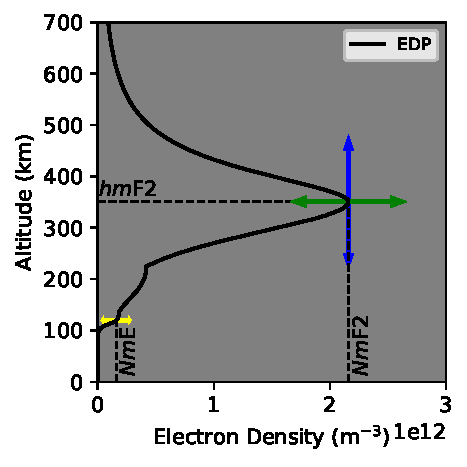
\includegraphics[scale=0.9]{PyIRI_EDP_components.pdf}
  \caption{Three anchor points control the shape of the electron density profile, where the peak of the F2 region is determined by the $Nm$F2 value, the height of the peak is determined by $hm$F2 parameter, and the peak of the E region is described by $Nm$E with fixed height.}
  \label{fig:EDP}
\end{figure}

%%%%%%%%%%%%%%%%%%%%%%%%%%%%%%%%%%%%%%%%%%%%%%%%%%%%%%%%%%%%%%%%%%%%%%%%%%%%%%%%%
\subsection{The peak of F2 region $Nm$F2: traditional IRI approach}\label{sec:F2}

The IRI model, as well as NeQuick \cite{Nav08} model, employs the Consultative Committee on International Radio (CCIR) coefficients to obtain the diurnal and geographical variations of the ionospheric critical frequency $fo$F2, whereas the $Nm$F2 is further derived from $fo$F2 using the plasma physics formula

\begin{equation}\label{eqn:freq2den}
Nm\mathrm{F2}/\mathrm{m^{-3}}=0.124\times 10^{11}(fo\mathrm{F2}/\mathrm{MHz})^2.
\end{equation}

The CCIR coefficients were obtained in the pioneered studies conducted by \citeA{Jon62, Jon65, Jon69}. They analyzed the monthly medians of the $fo$F2 for minimum and maximum levels of solar activity. First they found the coefficients for the Fourier time series to represent the diurnal trends of $fo$F2 at about 150 ionosonde stations using Least Squares minimization method. They, then, found the coefficients for a special set of geographic functions (similar to surface waves) to describe the variation of the found Fourier coefficients with geographic coordinates. As a result of their work, the diurnal and geographic variations of the monthly medians for $fo$F2 are described for 2 levels of solar activity using monthly sets of coefficients. 

In mathematical terms, the diurnal variations at a geographic latitude $\phi$ and East longitude $\theta$, and at a particular universal time (UT) $t$ expressed as angle time from $\pi$ to $-\pi$, the critical frequency can be expressed as
\begin{equation}\label{eqn:fourier}
fo\mathrm{F2}(\phi,\theta,t)=a_0(\phi, \theta)+\sum_{j=1}^{M}[a_{2i-1}(\phi, \theta)\cos(it)+a_{2i}(\phi, \theta)\sin(it)], 
\end{equation}
where the maximum number of the harmonics is $M=6$, and the geographic functions $a_i$ are defined as 
\begin{equation}\label{eqn:geographic}
a_i(\phi,\theta)=\sum_{j=0}^{J(0)}c_{i,j,0}P_{j,0}(\phi,\theta)+\sum_{k=1}^{8}\sum_{j=0}^{J(k)}(c_{i,j,2k-1}\cos(k\phi)+c_{i,j,2k}\sin(k\phi))\sin^j(\mu(\phi,\theta))\cos^k(\phi),
\end{equation}
where $\mu$ is a modified dip angle that can be calculated from the Earth magnetic inclination $I(\phi,\theta)$ as 
\begin{equation}\label{eqn:modip}
\mu=\tan^{-1}(I(\phi,\theta)/\cos(\phi)).
\end{equation}
The summation cutoffs $J(k)$ in Equation \ref{eqn:geographic} correspond to the truncation of the higher degrees of the latitudinal expansion, introduced by \citeA{Jon62} to reduce the noise of the median data points. Specifically, $J=[11, 11, 8, 4, 1, 0, 0, 0, 0]$ is employed for the $fo$F2. 

Coefficients $c$ in Equation \ref{eqn:geographic} for two levels of solar activity are provided as first 1976 numbers in 12 .asc files (one for each month) that accompany the IRI model. 

\begin{figure}[H]
  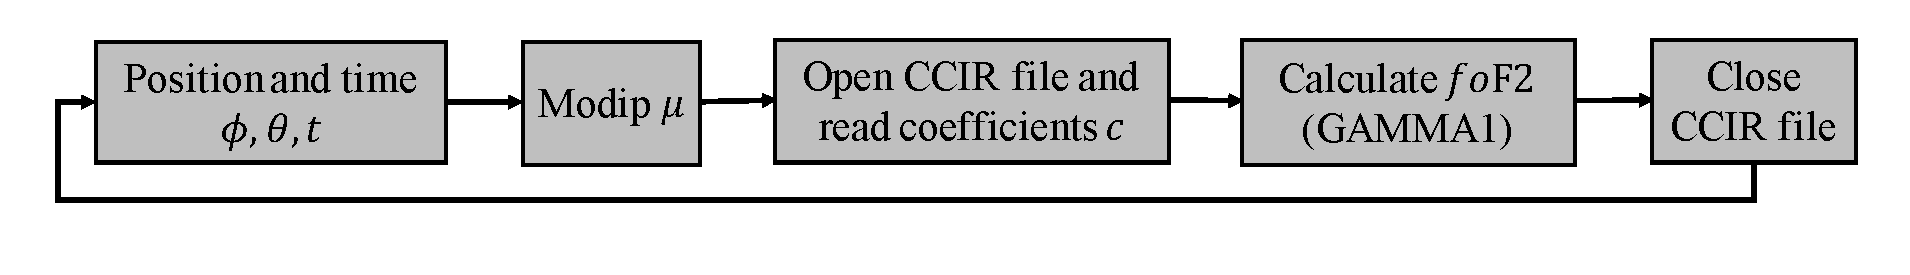
\includegraphics[scale=0.4]{IRI_flow.pdf}
  \caption{A simplified flow diagram of IRI model to obtain $fo$F2 from CCIR coefficients.}
  \label{fig:IRI_flow}
\end{figure}

In the IRI source code, a function called GAMMA1 calculates $fo$F2 following Equations \ref{eqn:fourier} and \ref{eqn:geographic}. The summation is obtained by sequential multiplication and addition of the coefficients with the functions inside of FORTRAN $do$ loops. A simplified version of the flow diagram for this process is shown in Figure \ref{fig:IRI_flow}. For a particular time $t$ and geographic position $(\phi, \theta)$, the modip $\mu$ is obtained, then the coefficients $c$ are read from the CCIR file and the function GAMMA1 is being called to calculate $fo$F2 following Equation \ref{eqn:fourier}. For the next time frame or for the next location of interest, this same process is repeated again and again. This scheme is simplified, dropping down the explanation of the interpolation between solar activity and the interpolation between 2 consequent monthly sets of coefficients. 

%%%%%%%%%%%%%%%%%%%%%%%%%%%%%%%%%%%%%%%%%%%%%%%%%%%%%%%%%%%%%%%%%%%%%%%%%%%%%%%%%
\section{The peak of F2 region $Nm$F2: Novel approach}\label{sec:F2}

In this section a novel approach to calculate $fo$F2 is described utilizing the fact that one CCIR set of coefficients contains all the necessary information to obtain the $fo$F2 simultaneously for the entire globe and for the entire diurnal range. 

The starting point begins with the formation of the position 1-D arrays $\Phi$ and $\Theta$ that specify the desired global grid with number of grid points $N_G$. These arrays can describe regular or irregular, global or regional grids. Similarly, the time of interest is specified as a 1-D array $T$. Python 3.7 International Geomagnetic Reference Field (IGRF-13) package \cite{Alk21} is employed for the calculation of the magnetic inclination $I$ for the given arrays $\Phi$ and $\Theta$, and the modip array $M$ is further calculated using Equation \ref{eqn:modip}.  
The global distribution of modip at zero altitude is shown in Figure \ref{fig:modip} for Apr 1, 2020. The modip distribution specifies where the magnetic equator is on the geographic coordinates. 

\begin{figure}[H]
  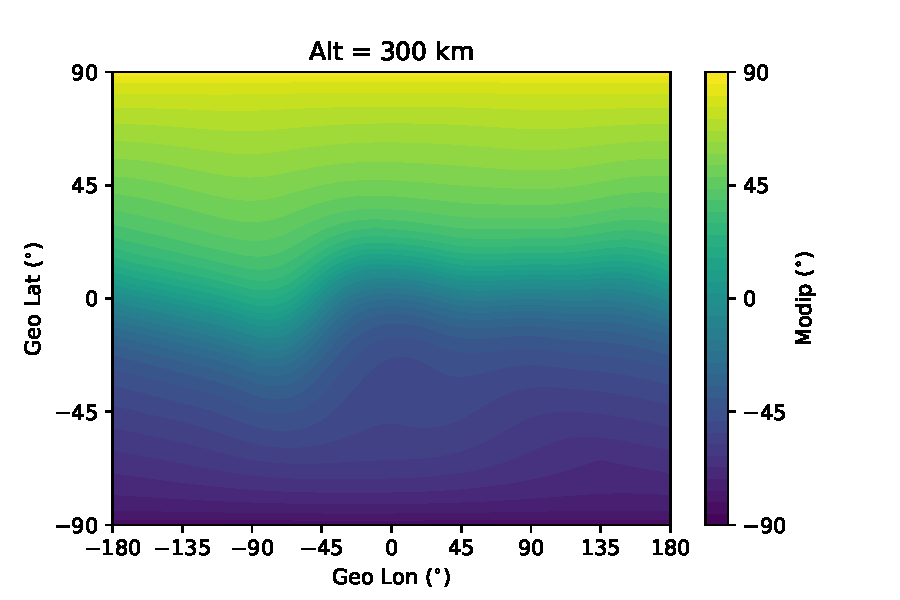
\includegraphics[scale=0.8]{PyIRI_modip.pdf}
  \caption{Example of the modified dip angle global distribution for Apr 1, 2020.}
  \label{fig:modip}
\end{figure}

Next, the Fourier functions are evaluated for the given time array $T$. Figure \ref{fig:diurnal} shows first two low order terms and the last high order terms of those functions, visualizing the highest level of the temporal resolution that can be achieved. A full list of functions is also shown on the right side of Figure \ref{fig:diurnal}. As a result of this step, a matrix of diurnal functions $F_D$ has $[N_T, 13]$ size, where $N_T$ is number of time steps.

\begin{figure}[H]
  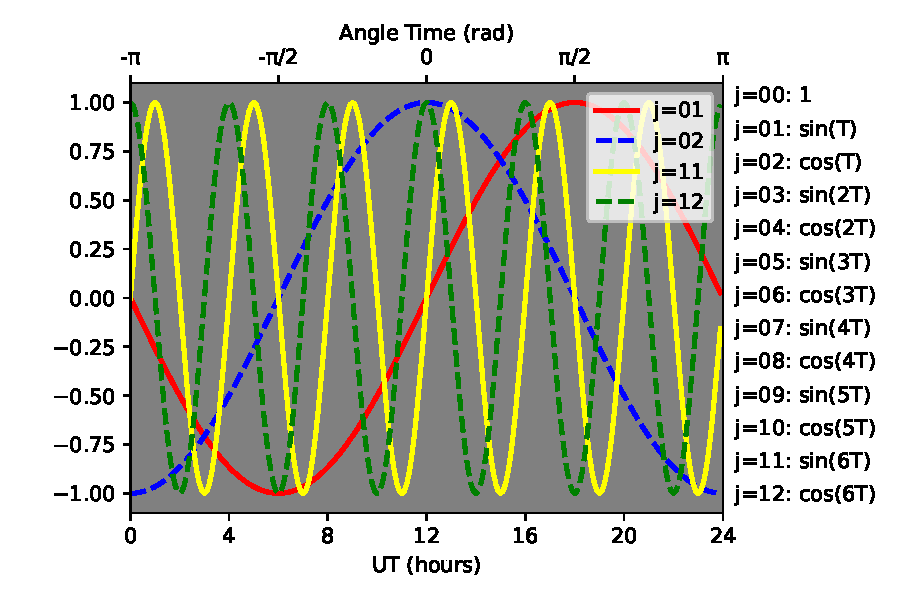
\includegraphics[scale=0.9]{NIDA_diurnal_functions.pdf}
  \caption{Few examples of the Fourier diurnal functions calculated for array of time spanned 24 hours of UT.}
  \label{fig:diurnal}
\end{figure}

Further, the global functions are evaluated for the positional arrays $\Phi$, $\Theta$, and the array of modip $M$. Capital Greek letters are used to emphasize that these are the arrays and not the single numbers. Figure \ref{fig:global} shows several examples of the global functions. The main difference from regular spherical harmonics is the modip dependency, that can be clearly visible from the first function shown in Figure \ref{fig:global}a. The smallest ionospheric structures that can be revealed by the highest expansion term is shown in Figure \ref{fig:global}l. Additionally, the list of all $76$ global functions is shown on the right of Figure \ref{fig:global}. As a result of this step, a matrix of global functions $F_G$ has $[76, N_G]$ elements, where $N_G$ is number of grid points.

\begin{figure}[H]
  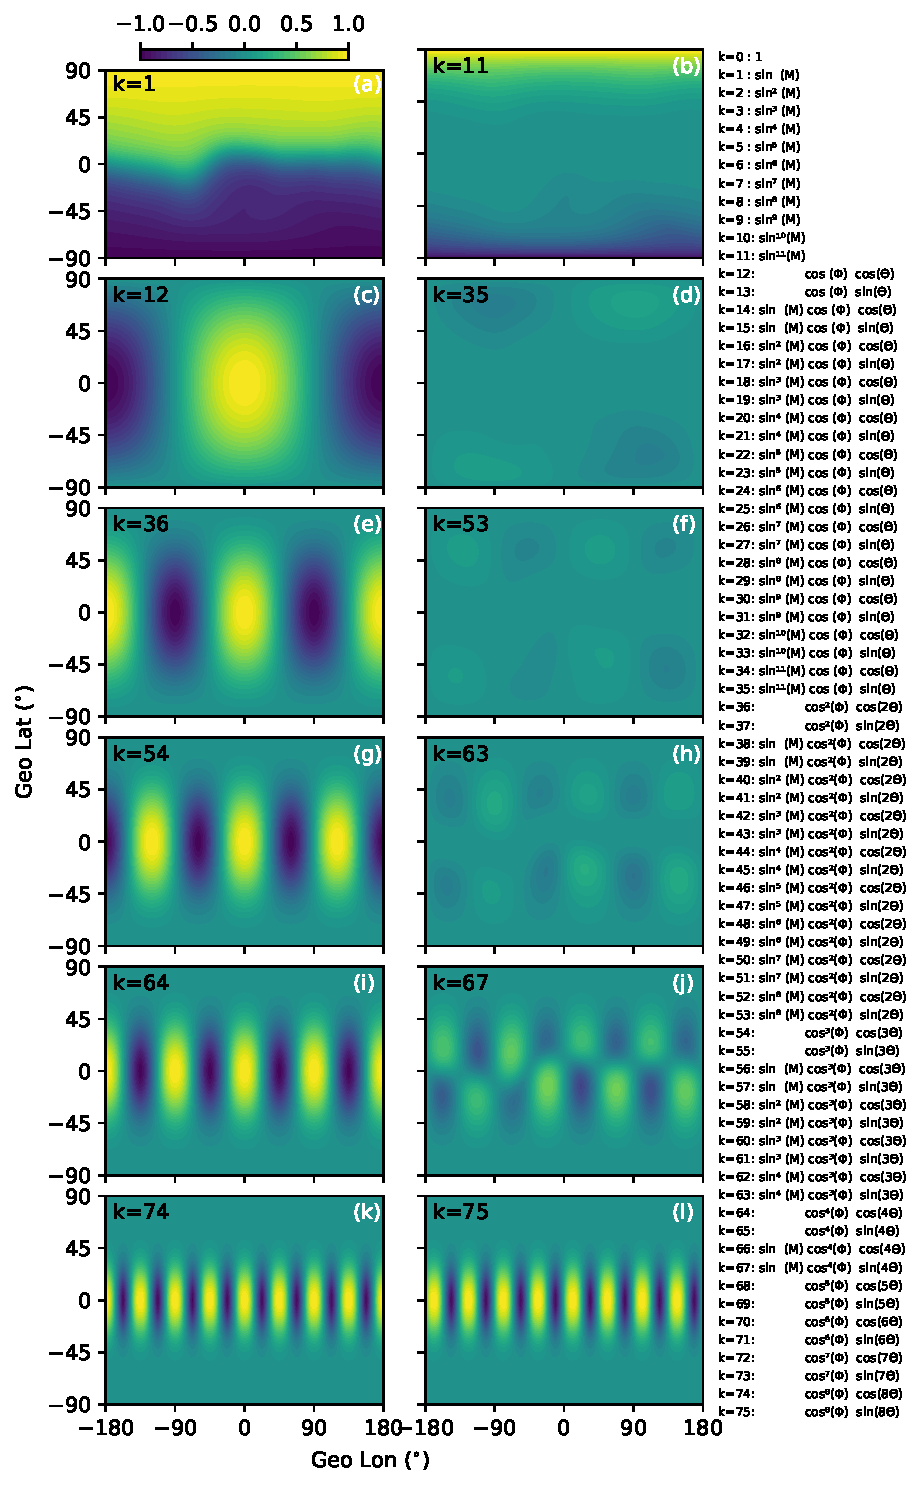
\includegraphics[scale=0.99]{Global_functions.pdf}
  \caption{Few examples of the global functions calculated for the array of grid points. The list of all functions is shown on the right.}
  \label{fig:global}
\end{figure}

Then, the 1-D array of CCIR coefficients $c$ that has 1976 elements can be reformed into a matrix $U$ of size $[13, 76, 2]$, where the first dimension corresponds to 13 Fourier series, the second dimension represents 76 global functions, and the third dimension represents the 2 levels of solar activity. For one level of solar activity matrix $U$ is reduced to size $[13, 76]$.

Finally, a matrix multiplication operation 
\begin{equation}\label{eqn:modip}
fo\mathrm{F2}=(F_D U)F_G
\end{equation}
gives a critical frequency $fo\mathrm{F2}$ matrix with size $[N_T, N_G]$, which is further converted to $Nm\mathrm{F2}$ using Equation \ref{eqn:freq2den}. 

An example of the $Nm\mathrm{F2}$ output for 2 levels of solar activity is shown in Figure \ref{fig:NmF2_min_max} for 10 UT of April 15, 2020. The location of the subsolar point is shown with red circle. For the solar minimum, the CCIR coefficients were derived using data from 1954-1955, and for the solar maximum the years 1956-1958 were considered \cite{Jon62, Jon65, Jon69}. 

\begin{figure}[H]
  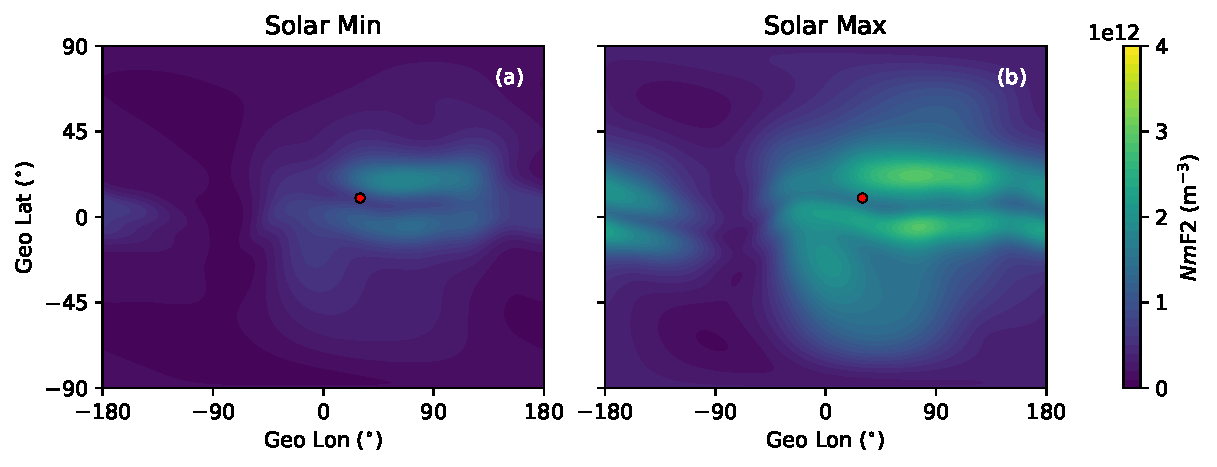
\includegraphics[scale=0.7]{PyIRI_NmF2_min_max.pdf}
  \caption{Peak of electron density $Nm\mathrm{F2}$ for solar minimum (a) and solar maximum (b) for 10 UT of April 2020. Red circle shows the location of subsolar point.}
  \label{fig:NmF2_min_max}
\end{figure}

A simplified version of the flow diagram for the PyIRI code is shown in Figure \ref{fig:PyIRI_flow}. In summary, the global functions $F_G$ are calculated for 3 arrays $\Phi$, $\Theta$, and $M$, and the Fourier functions $F_T$ are calculated for a time array $T$. The CCIR coefficients are stored in matrix $U$, and the multiplication between $F_D$, $U$, and $F_G$ gives $fo\mathrm{F2}$ for the entire grid and for the entire time array. Importantly, this one operation substitutes $6,272,736$ executions of the IRI FORTRAN code in case of global regular grid of $1^{\circ} \times 1^{\circ}$ and 15-min-resolution temporal array. 

\begin{figure}[H]
  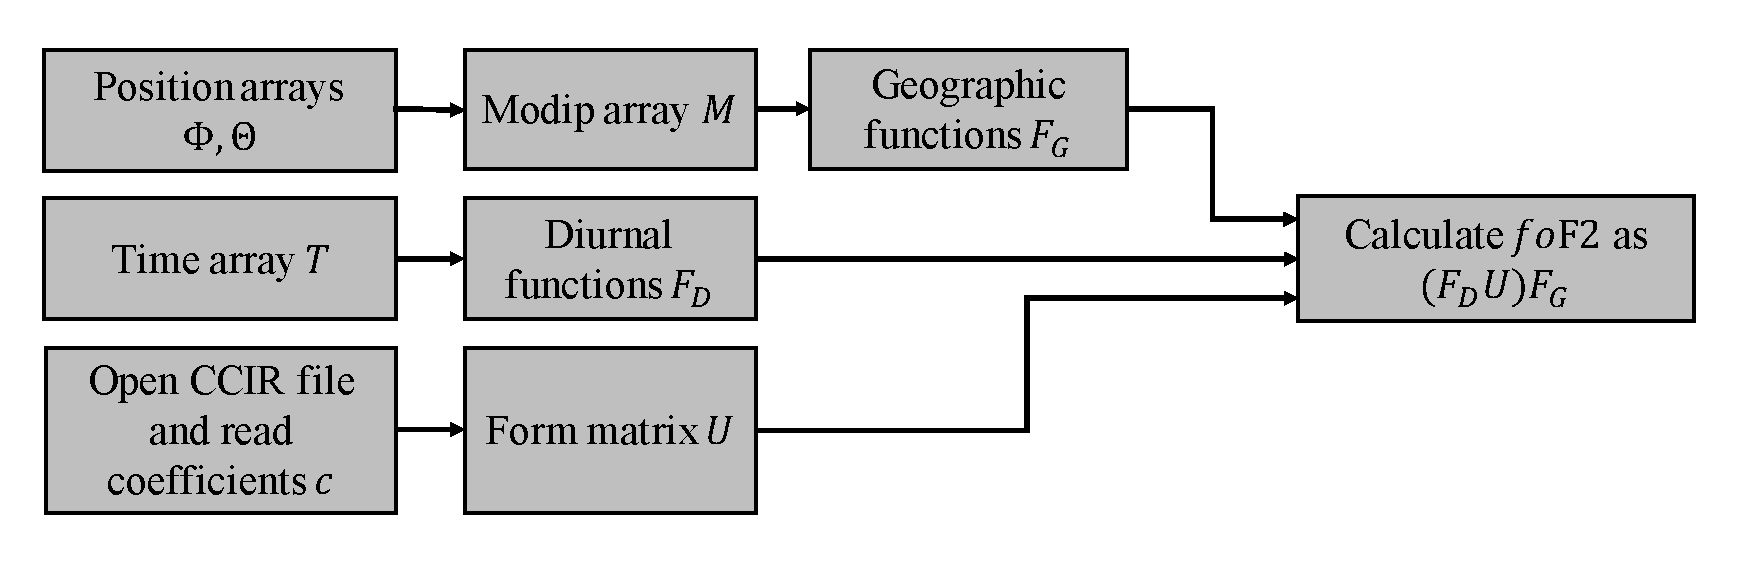
\includegraphics[scale=0.5]{PyIRI_flow.pdf}
  \caption{A simplified flow diagram for the PyIRI code to obtain $fo$F2 from CCIR coefficients.}
  \label{fig:PyIRI_flow}
\end{figure}

%%%%%%%%%%%%%%%%%%%%%%%%%%%%%%%%%%%%%%%%%%%%%%%%%%%%%%%%%%%%%%%%%%%%%%%%%%%%%%%%%%%%%%%%
\section{The height of F2 peak $hm$F2}\label{subsec:hmF2}
The CCIR files also contain 882 coefficients (following first 1976 coefficients for $fo\mathrm{F2}$) that correspond to the $\mathrm{MUF(3000)F2}/fo\mathrm{F2}$, where
$\mathrm{MUF(3000)F2}$ is the highest frequency that is refracted in the ionosphere and can be received at a distance of 3,000 km. The only difference between the calculation of $fo\mathrm{F2}$ and $\mathrm{MUF(3000)F2}/fo\mathrm{F2}$ is in the number of the global and diurnal functions. In the case of $\mathrm{MUF(3000)F2}/fo\mathrm{F2}$, the truncation is determined by $J=[6, 7, 5, 2, 1, 0, 0]$ and gives 49 geographic functions, whereas 9 Fourier functions are used. Therefore, the matrix with the CCIR coefficients has $[9, 49, 2]$ size. Figure \ref{fig:M3000_min_max} shows $\mathrm{MUF(3000)F2}/fo\mathrm{F2}$ for minimum and maximum solar activity calculated from CCIR coefficients for April of 2020, 10 UT. 

\begin{figure}[H]
  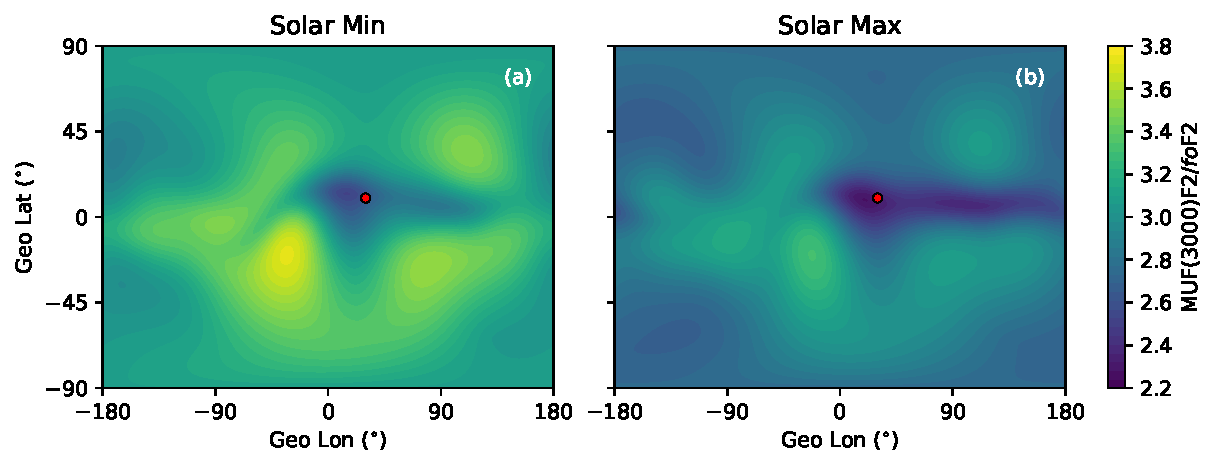
\includegraphics[scale=0.7]{PyIRI_M3000_min_max.pdf}
  \caption{CCIR $\mathrm{MUF(3000)F2}/fo\mathrm{F2}$ for solar minimum (a) and solar maximum (b) for 10 UT of April 2020. Red circle shows the location of subsolar point.}
  \label{fig:M3000_min_max}
\end{figure}

Further, following BSE-1979 option of IRI \cite{Bil22}, developed by \citeA{Bil79} the $hm$F2 parameter is derived as
\begin{equation}\label{eqn:hmf2}
hm\mathrm{F2}=\frac{1490}{\mathrm{MUF(3000)F2}/fo\mathrm{F2}+DM}-176,
\end{equation}
where the correction factor DM is 
\begin{equation}\label{eqn:DM}
DM=\frac{f_1 f_2}{\frac{fo\mathrm{F2}}{fo\mathrm{E}}-f_3}+f_4,
\end{equation}
and the following functions $f$ depend on 12-month running mean of sunspot number $R_{12}$ and on modip array $M$
\begin{equation}\label{eqn:f1}
f_1=0.00232R_{12}+0.222,
\end{equation}
\begin{equation}\label{eqn:f2}
f_2=1-\frac{R_{12}}{150}\exp\left[ -\left(\frac{M}{40}\right)^2\right],
\end{equation}
\begin{equation}\label{eqn:f3}
f_3=1.2-0.0116\exp\left(\frac{R_{12}}{41.84}\right),
\end{equation}
\begin{equation}\label{eqn:f4}
f_4=0.096\frac{R_{12}-25}{150}.
\end{equation}
An additional limit is added to ratio $\frac{fo\mathrm{F2}}{fo\mathrm{E}}$, where it is fixed at 1.7 in case it goes below 1.7. 

After applying Equation \ref{eqn:hmf2}, the height of the F2 region peak is shown in Figure \ref{fig:hmF2_min_max}. 
\begin{figure}[H]
  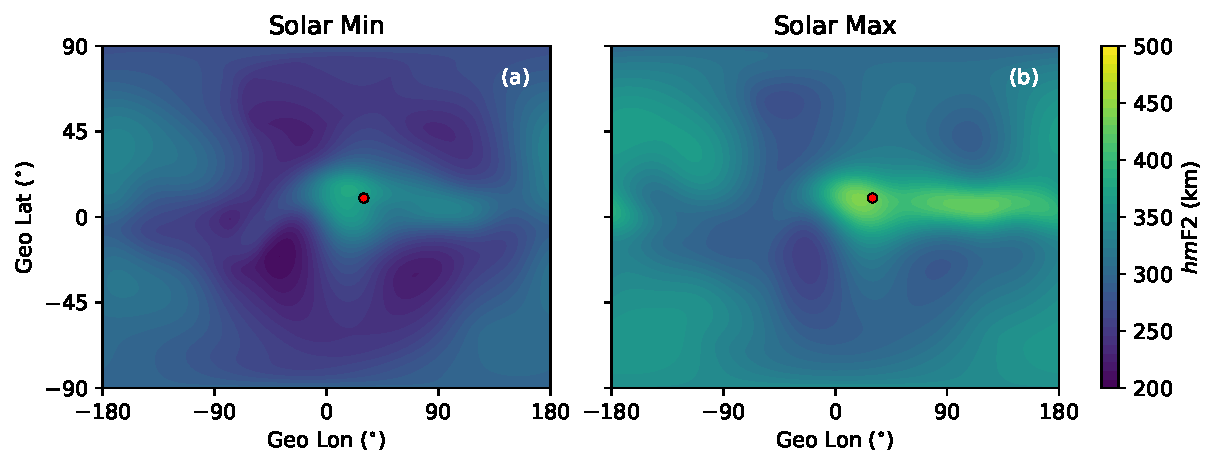
\includegraphics[scale=0.7]{PyIRI_hmF2_min_max.pdf}
  \caption{Height of the electron density peak $hm\mathrm{F2}$ for solar minimum (a) and solar maximum (b) for 10 UT of April 2020. Red circle shows the location of subsolar point.}
  \label{fig:hmF2_min_max}
\end{figure}

%%%%%%%%%%%%%%%%%%%%%%%%%%%%%%%%%%%%%%%%%%%%%%%%%%%%%%%%%%%%%%%%%%%%%%%%%%%%%%%%%%%%%%%%
\section{E region parameters}\label{sec:NmE}
The E region model for this version of PyIRI was chosen to be somewhat simpler than the one used in the source code of IRI, following the approach from NeQuick model. First the effective solar zenith angle is being calculated as
\begin{equation}\label{eqn:effective_sz}
\Psi_{eff}=\frac{\Psi+ \left[ 90-0.24\exp(20-0.2\Psi) \right]\exp(12(\Psi-\Psi_0))}{1+\exp(12(\Psi-\Psi_0))},
\end{equation}
where $\Psi$ is a solar zenith angle, and $\Psi_0$ is a solar zenith angle at day night transition, which is set to 86.23292796211615$^{\circ}$. 

Further a seasonal parameter $s$ is defined as 
\begin{equation}\label{eqn:s}
s=s_0 \left(\frac{\exp(0.3\Phi)-1}{\exp(0.3\Phi)+1}\right),
\end{equation}
with $s_0$ being month dependent
\begin{equation}\label{eqn:s}
s_0 =
\left\{ 
\begin{array}{l}-1, \quad \mathrm{month} = 1,2,11,12, \\ 
0, \quad \quad \mathrm{month} = 3,4,9,10, \\ 
1, \quad \quad \mathrm{month} = 5,6,7,8. 
\end{array} 
\right.
\end{equation}

The critical frequency of E region is then calculated using 
\begin{equation}\label{eqn:foE}
fo\mathrm{E}=\sqrt{0.49+(1.112-0.019s)^2\sqrt{\mathrm{F10.7}} \cos^{0.6}(\Psi_{eff})},
\end{equation}
where $\mathrm{F10.7}$ is the solar radio flux at 10.7 cm, and $\Psi_{eff}$ is converted to radians. 

Figure \ref{fig:foE_min_max} shows the $E$-region critical frequency for 2 levels of solar activity for 10 UT of April 2020. The climatology of E region is mainly controlled by the solar ionization and therefore depends on the location of subsolar point, shown with red circle in Figure \ref{fig:foE_min_max}.  

\begin{figure}[H]
  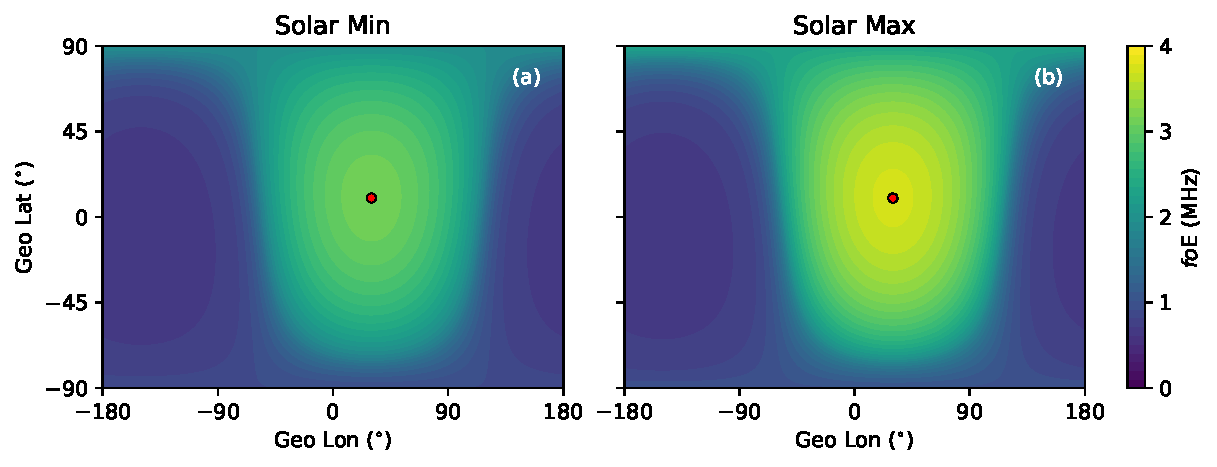
\includegraphics[scale=0.7]{PyIRI_foE_min_max.pdf}
  \caption{$fo\mathrm{E}$ for solar minimum (a) and solar maximum (b) for 10 UT of April 2020. Red circle shows the location of subsolar point.}
  \label{fig:foE_min_max}
\end{figure}

Additionally, the height of the E region $hmE$ is assumed to be fixed at 110 km, with the thickness of the bottom side of E region $B^{E}_{bot}$ being fixed at 5 km, and $B^{E}_{top}$ being fixed at 7 km. 


%%%%%%%%%%%%%%%%%%%%%%%%%%%%%%%%%%%%%%%%%%%%%%%%%%%%%%%%%%%%%%%%%%%%%%%%%%%%%%%%%%%%%%%%
\section{Thicknesses of the ionospheric layers}\label{sec:thicknesses}
This version of the PyIRI code has simplified approach to the construction of the ionospheric profile, in comparison to the standard IRI source code and its options. For the thickness of bottom side of F2 region, an approach similar to NeQuick model is chosen, where the bottom side is being described by Epstein function, that has one parameter that describes it's thickness, unlike the IRI model, where two parameters $B_0$ and $B_1$ are employed. 

\subsection{Thickness of the bottom side of the F2 layer $B^{\mathrm{F2}}_{bot}$}\label{sec:B_F2_bot}
The thickness of the bottom layer in PyIRI is modeled as a function of $fo\mathrm{F2}$ and $\mathrm{MUF(3000)F2}/fo\mathrm{F2}$ as
\begin{equation}\label{eqn:B_F2_bot}
B^{\mathrm{F2}}_{bot}=\frac{47.74 \quad fo\mathrm{F2}^2 }{\exp(-3.467+1.714\ln(fo\mathrm{F2})+2.02\ln(\mathrm{MUF(3000)F2}/fo\mathrm{F2}))},
\end{equation}
and is shown in Figure \ref{fig:BF2_bot_min_max} for 2 levels of solar activity.

\begin{figure}[H]
  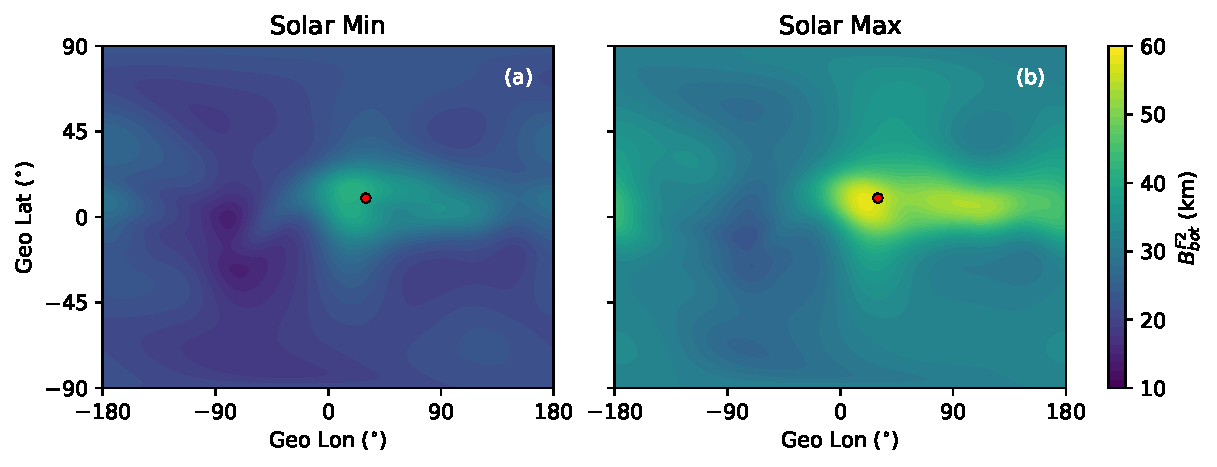
\includegraphics[scale=0.7]{PyIRI_B_F2_bot_min_max.pdf}
  \caption{Thickness of the bottom side of F2 region $B^{\mathrm{F2}}_{bot}$ for solar minimum (a) and solar maximum (b) for 10 UT of April 2020. Red circle shows the location of subsolar point.}
  \label{fig:BF2_bot_min_max}
\end{figure}

\subsection{Thickness of the top side of the F2 layer} 
IRI model provides three different options to define the thickness of the top side of F2 layer $B^{F2}_{top}$, with the NeQuick approach being the standard option. However, there are slight differences in the definitions $B^{F2}_{top}$ in NeQuick and IRI code. Here we define $B^{F2}_{top}$ the following way, combining the two approaches: 
\begin{equation}\label{eqn:B_F2_top}
B^{\mathrm{F2}}_{top}=\frac{100x+150}{0.041163x^2-0.183981x+1.424472},
\end{equation}
where $x$ depends on $B^{\mathrm{F2}}_{bot}$
\begin{equation}\label{eqn:x}
x=\frac{k B^{\mathrm{F2}}_{bot}-150}{100},
\end{equation}
with shape parameter $k$ defined as
\begin{equation}\label{eqn:k}
k=3.22-0.0538 fo\mathrm{F2}-0.00664 hm\mathrm{F2} +0.113 \frac{hm\mathrm{F2}}{B^{\mathrm{F2}}_{bot}}+0.00257 R_{12}.
\end{equation}
In NeQuick definition of $k$, the dependence on the solar activity is expressed in terms of effective ionization level, whereas in IRI the 12-month running-mean of sunspot number $R_{12}$ is used.
The $B^{\mathrm{F2}}_{top}$ is shown in Figure \ref{fig:BF2_top_min_max} for 2 levels of solar activity.

\begin{figure}[H]
  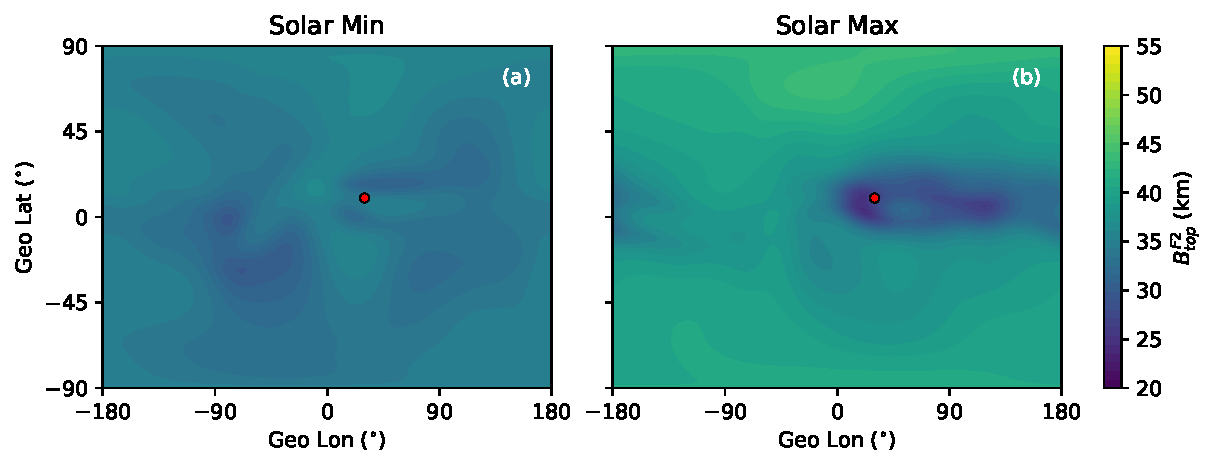
\includegraphics[scale=0.7]{PyIRI_B_F2_top_min_max.pdf}
  \caption{Thickness of the top side of F2 region $B^{\mathrm{F2}}_{top}$ for solar minimum (a) and solar maximum (b) for 10 UT of April 2020. Red circle shows the location of subsolar point.}
  \label{fig:BF2_top_min_max}
\end{figure}

%%%%%%%%%%%%%%%%%%%%%%%%%%%%%%%%%%%%%%%%%%%%%%%%%%%%%%%%%%%%%%%%%%%%%%%%%%%%%%%%%%%%%%%%
\section{F1 region parameters}
The F1 region appears only during the day time. It's occurrence probability function 
\begin{equation}\label{eqn:P}
P=\left(0.5+0.5\cos(\Psi)\right)^{2.36},
\end{equation}
was chosen not to depend on $R_{12}$ and magnetic latitude, following the suggestion in \citeA{Bil22}. The distribution of $P$ is shown in Figure \ref{fig:foF1_min_max}a, with the color bar shown on the right of the figure. It's global distribution is very similar to the $NmE$ distribution, indicating strong solar control. Further, when the occurrence probability is greater than 0.5, the critical frequency of F1 layer can be modeled as
\begin{equation}\label{eqn:foF1}
fo\mathrm{F1}=f_s\cos^n(\Psi),
\end{equation}
where
\begin{equation}\label{eqn:foF1_components}
\begin{array}{l}f_s=f_0+\frac{(f_{100}-f_{0})R_{12}}{100}, \\
f_0=4.35+0.0058|M'|-0.00012M'^2, \\
f_{100}=5.348+0.011|M'|-0.00023M'^2, \\
n=0.093+0.0046|M'|-0.000054M'^2+0.0003R_{12}, \\
M'=\tan^{-1}(\frac{1}{2}\tan(M)),
\end{array} 
\end{equation}
with $M'$ being magnetic dip latitude, that can be calculated from modified dip angle matrix $M$.
Figures \ref{fig:foF1_min_max}b and \ref{fig:foF1_min_max}c show the critical frequency $fo$F1 during solar minimum and solar maximum, respectively, for 10 UT of April 2020.

\begin{figure}[H]
  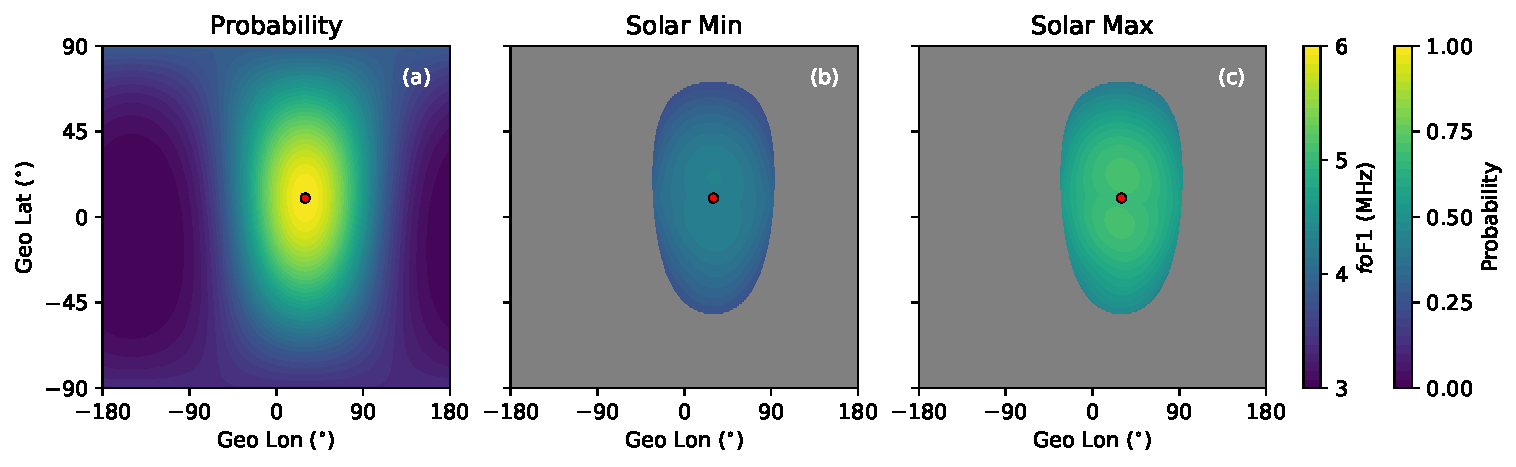
\includegraphics[scale=0.6]{PyIRI_foF1_min_max.pdf}
  \caption{Occurrence probability function $P$ for F1 region (a), with critical frequency $fo$F1 during solar minimum (b) and solar maximum (c) for 10 UT of April 2020. Red circle shows the location of subsolar point.}
  \label{fig:foF1_min_max}
\end{figure}

The height of the F1 layer $hm$F1 is found where the bottom side of F2 layer drops to the value of $fo$F1, in case when F1 layer is present. This height is found analytically using the following expression derived from Epstein function
\begin{equation}\label{eqn:hmF1}
hm\mathrm{F1}=B^{\mathrm{F2}}_{bot}\log\left(-\left(1-\frac{2Nm\mathrm{F2}}{Nm\mathrm{F1}}\right)-\sqrt{\left(1-\frac{2Nm\mathrm{F2}}{Nm\mathrm{F1}}\right)^2-1}\right)+hm\mathrm{F2}.
\end{equation}
The $hm$F1 map is shown in Figure \ref{fig:hmF1_min_max}.
\begin{figure}[H]
  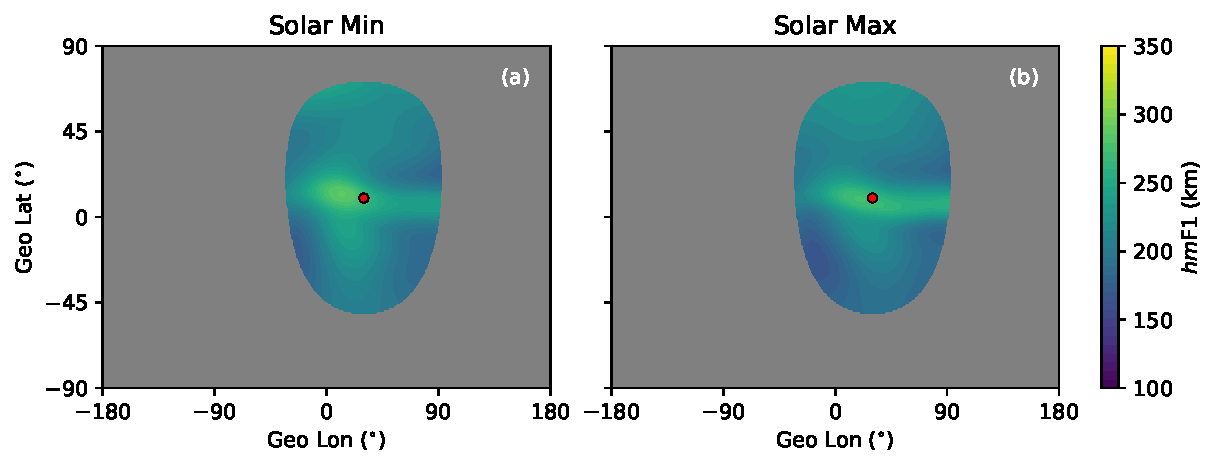
\includegraphics[scale=0.7]{PyIRI_hmF1_min_max.pdf}
  \caption{F1 region peak height $hm$F1 during solar minimum (a) and solar maximum (b) for 10 UT of April 2020. Red circle shows the location of subsolar point.}
  \label{fig:hmF1_min_max}
\end{figure}

A regular Epstein function is employed to model the bottom side of F1 region, with the following thickness
\begin{equation}\label{eqn:foF1}
B^{\mathrm{F1}}_{bot}=0.5(hm\mathrm{F1}-hm\mathrm{E}),
\end{equation}
that is also shown in Figure \ref{fig:BF1_bot_min_max}.

\begin{figure}[H]
  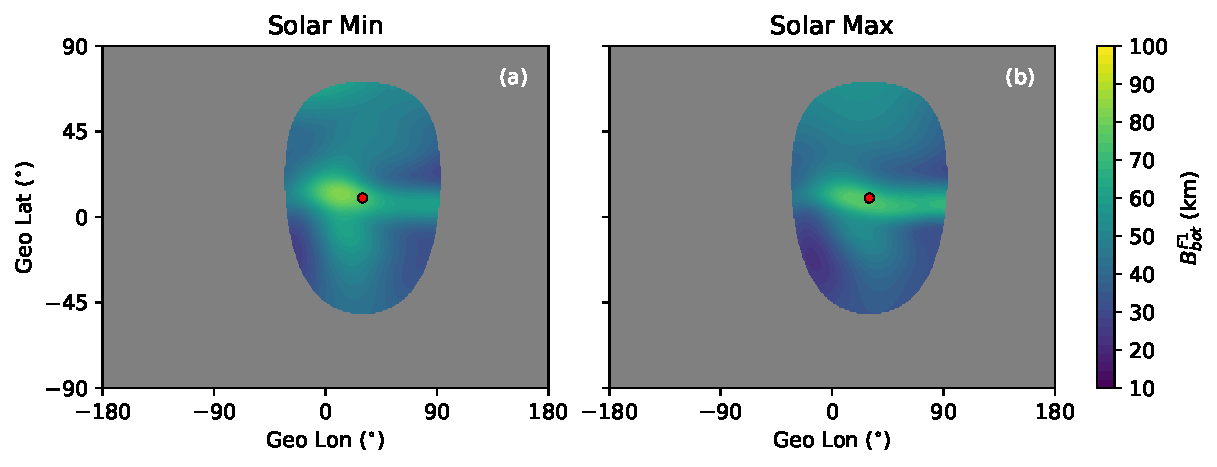
\includegraphics[scale=0.7]{PyIRI_B_F1_bot_min_max.pdf}
  \caption{Thickness of the bottom side of F1 region $B^{\mathrm{F1}}_{bot}$ for solar minimum (a) and solar maximum (b) for 10 UT of April 2020. Red circle shows the location of subsolar point.}
  \label{fig:BF1_bot_min_max}
\end{figure}

%%%%%%%%%%%%%%%%%%%%%%%%%%%%%%%%%%%%%%%%%%%%%%%%%%%%%%%%%%%%%%%%%%%%%%%%%%%%%%%%%%%%%%%%
\section{Sporadic E layer $Es$}
PyIRI also includes monthly mean of the sporadic E layer $Es$, using mean monthly coefficients \cite{Bra03}. They are in the same format as CCIR coefficients, but with different truncation of the higher degrees of the latitudinal expansion $J=[10, 12, 6, 2, 0, 0]$. Figure \ref{fig:Es_min_max} shows the critical frequency of the sporadic E layer $Es$ for both levels of solar activity. 
\begin{figure}[H]
  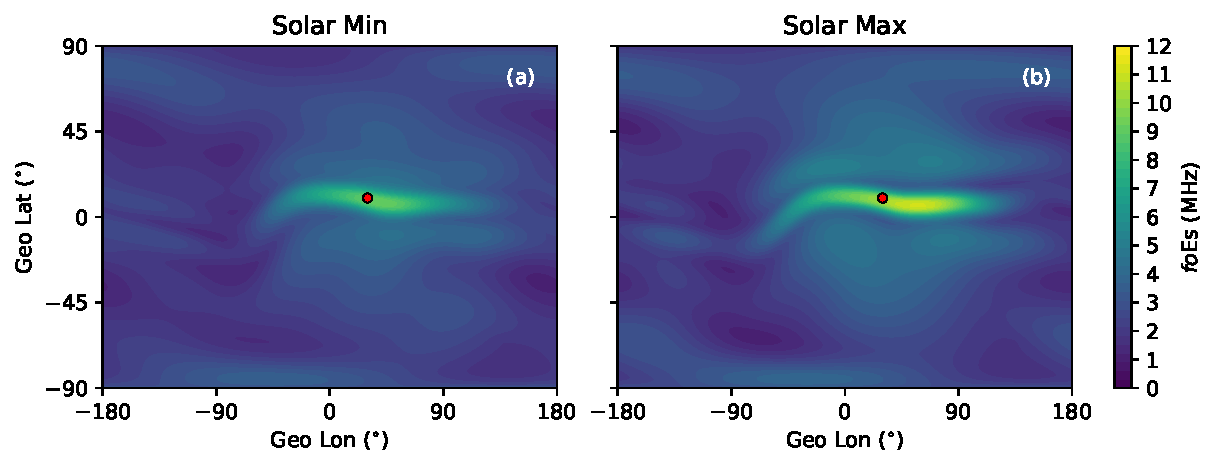
\includegraphics[scale=0.7]{PyIRI_foEs_min_max.pdf}
  \caption{Critical frequency of the sporadic E layer $Es$ for solar minimum (a) and solar maximum (b) for 10 UT of April 2020. Red circle shows the location of subsolar point.}
  \label{fig:Es_min_max}
\end{figure}
This parameter, however, is not included in the construction of the vertical electron density profile, described in the following section. 

%%%%%%%%%%%%%%%%%%%%%%%%%%%%%%%%%%%%%%%%%%%%%%%%%%%%%%%%%%%%%%%%%%%%%%%%%%%%%%%%%%%%%%%%
\section{Construction of the 3-D ionosphere from the maps of the parameters}
This section explains how the 3-D ionosphere is constructed form the maps of the ionospheric parameters. This approach was specifically developed for PyIRI. 

First, let's consider a 1-D example of the profile construction from the set of coefficients. 
The coefficients were chosen from the $\phi=0^{\circ}$ and $\theta=100^{\circ}$ location, where the F1 region is not present, for solar maximum condition. Figure \ref{fig:EDP_no_F1}a shows the $Nm\mathrm{F2}$ and $Nm\mathrm{E}$ parameters with red and purple circles, located at the $hm\mathrm{F2}$ and $hm\mathrm{E}$ heights, respectively. 

\begin{figure}[H]
  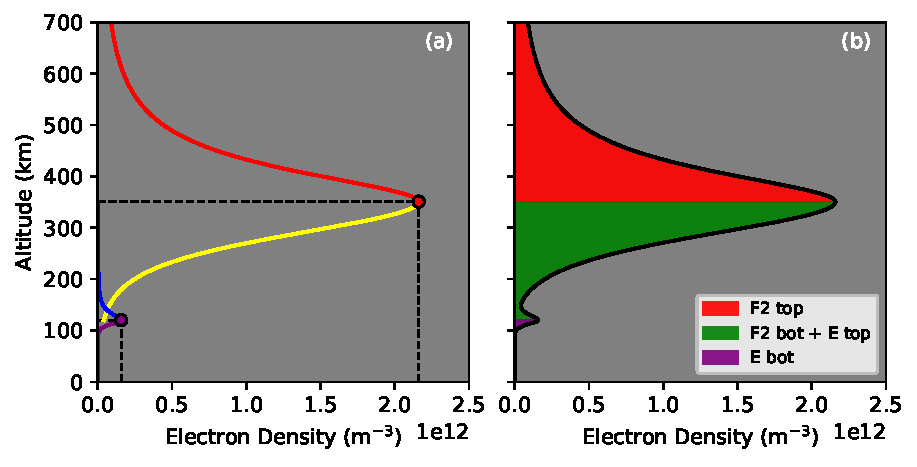
\includegraphics[scale=0.9]{Construction_of_EDP_without_F1.pdf}
  \caption{Construction of the EDP without F1 region.}
  \label{fig:EDP_no_F1}
\end{figure}

The bottom side of the F2 region, the topside of E region, and the bottom side of E region, shown with yellow, blue, and purple colors in Figure \ref{fig:EDP_no_F1}a are constructed using Epstein function 
\begin{equation}\label{eqn:Epstein}
Ne=4Nm\frac{e^{\frac{h-hm}{B}}}{\left(1-e^{\frac{h-hm}{B}}\right)^2},
\end{equation}
using corresponding peak densities $Nm$, heights of the peaks $hm$, and thicknesses $B$. The bottom side of F2 region is evaluated from $hm\mathrm{F2}$ down to $hm\mathrm{E}$. The topside of E region is evaluated from $hm\mathrm{E}$ up to $hm\mathrm{F2}$. Further, the top side of the F2 region, shown with red in Figure \ref{fig:EDP_no_F1} is calculated using Equation  \ref{eqn:Epstein}, with the modified thickness of the profile
\begin{equation}\label{eqn:B_modified}
B_{modified}=B^{\mathrm{F2}}_{top}\left(1+\frac{12.5(h-hm\mathrm{F2})}{100B^{\mathrm{F2}}_{top}+0.125(h-hm\mathrm{F2})}\right).
\end{equation}
A special care needs to be taken for the region between $hm\mathrm{F2}$ and $hm\mathrm{E}$ to add two curves together. Unlike in IRI and NeQuick, a drop function was introduce to model the transition of E region to the F2 region, without any re-scaling of the peaks. A drop function of the following form was implemented
\begin{equation}\label{eqn:drop}
Y_{up}=1-\left(\frac{h-hm\mathrm{E}}{hm\mathrm{F2}-hm\mathrm{E}}\right)^4.
\end{equation}
Prior to the summation, the topside of E region is multiplied by $Y_{up}$ and the bottom side of $F2$ is multiplied by  
\begin{equation}\label{eqn:drop}
Y_{down}=1-\left(\frac{hm\mathrm{F2}-h}{hm\mathrm{F2}-hm\mathrm{E}}\right)^4.
\end{equation}
Since the contribution of the E region is minimal above 150 km, the shape of the bottom side F2 region remains unchanged, but the influence of the F2 region on the topside of E region will be reduced. Figure \ref{fig:EDP_no_F1}b shows the final profile with different regions indicated by the color. 

In case when the F1 region is present, like at the location with $\phi=0^{\circ}$ and $\theta=0^{\circ}$, the bottom side of F1 region is modeled as an Epstein function, and the bottom of the F2 region is not extended further than $hm\mathrm{F1}$. The same drop function is used to reduce the influence of F1 region on the top side of E region and the influence of the top of E region on the bottom of F1 region prior to their summation. Figure \ref{fig:EDP_yes_F1}a shows the $Nm\mathrm{F1}$ with orange circle and the bottom of the F1 region with yellow curve. As can be seen in Figure \ref{fig:EDP_yes_F1}b, the drop function approach works well to merge the 2 regions without changing the shapes of the individual regions and without any re-scaling of the peaks. 

\begin{figure}[H]
  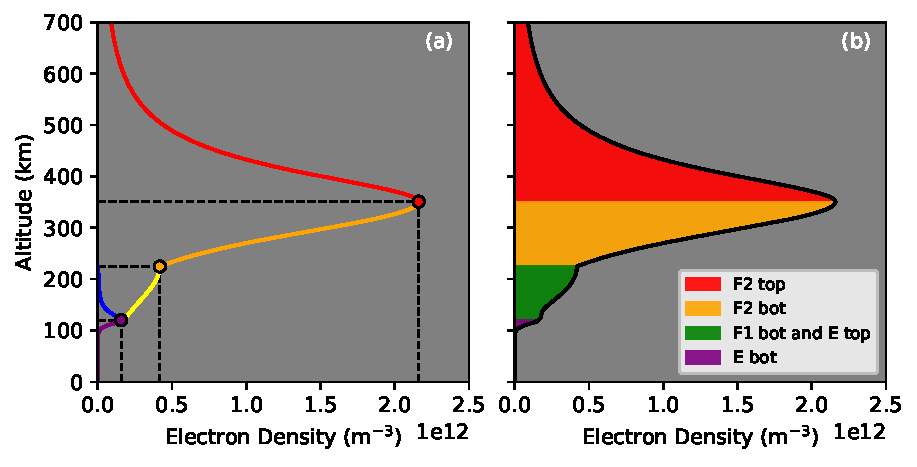
\includegraphics[scale=0.9]{Construction_of_EDP_with_F1.pdf}
  \caption{Construction of the EDP with F1 region.}
  \label{fig:EDP_yes_F1}
\end{figure}



It is important to mention, that even if the computation time was dramatically reduced to construct the maps of $Nm\mathrm{F2}$ and $hm\mathrm{F2}$ from the CCIR coefficients and to further derive all the other parameters in matrix form, it would still be computationally expensive to build the profiles in the traditional way, by doing it for each horizontal position. In this case, a particular function that constructs the profiles from the set of coefficients would need to be (again, on top of the derivation of the parameters) called $6,272,736$ times in case of the global regular grid of $1^{\circ} \times 1^{\circ}$ and 15-min-resolution temporal array. 

This problem, however, can be solved with the help of Python $numpy.where$ function in NumPy package that can have not only multidimensional argument, but also a multidimensional condition. Figure \ref{fig:surface} helps to visualize this 2-D selection, where red, orange, and purple surfaces show $hm\mathrm{F2}$, $hm\mathrm{F1}$, and $hm\mathrm{E}$, respectively. These surfaces represent the boundaries for the selection, similar to 1-D example with red, orange and purple circles in Figure \ref{fig:EDP_yes_F1}a. For example, to construct the topside of the ionosphere simultaneously for the entire global grid, all 3-D grid points that are located above the red surface need to be selected and passed to the Epstein function. Similarly, to construct the bottom side of the F2 region, when the F1 region is present, all the points between the green and red surfaces should be selected. 
The trick to make a 2-D selection is to present all parameters as 2-D matrices, by populating the same information at all heights. For example, a matrix for $hm\mathrm{F2}$ will have $[N_G, N_V]$ size, where $N_V$ is the number of desired vertical grid cells that correspond to an array of altitudes $h$. This matrix will have same elements at all $N_V$. Same should be done for all other parameters. However, the height matrix $H$ should have $[N_V, N_G]$ elements, with the heights being equal at all horizontal locations. Further, the output of $numpy.where(H \ge hm\mathrm{F2})$ gives 2-D indexes for the location of all the grid cells that correspond to the ionospheric top side of F2 region $IND_{top}^{\mathrm{F2}}$. Finally, $Nm\mathrm{F2}[IND_{top}^{\mathrm{F2}}]$, $hm\mathrm{F2}[IND_{top}^{\mathrm{F2}}]$, $B^{\mathrm{F2}}_{top}[IND_{top}^{\mathrm{F2}}]$, and $H[IND_{top}^{\mathrm{F2}}]$ can be given to the topside Epstein function using Equations \ref{eqn:Epstein} and \ref{eqn:B_modified} to perform the calculation of the electron density for the top side of the F2 region. The result will have the same shape $[N_G, N_V]$ as the input.

Additionally, it is not necessary to introduce a separate dimension for time with size $N_T$. Instead, all the matrices can have $[N_G\times N_T, N_V]$ shape and the final outputs can be further reshaped to $[N_T, N_G, N_V]$. 

\begin{figure}[H]
  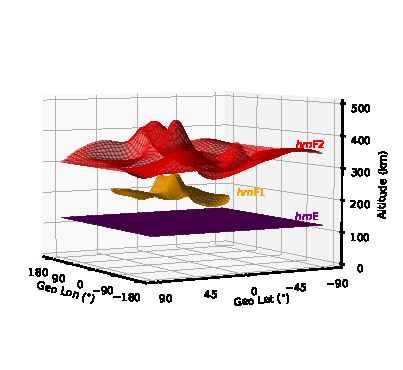
\includegraphics[scale=2]{PyIRI_3D_hm_limits.pdf}
  \caption{Surfaces of $hm\mathrm{F2}$, $hm\mathrm{F1}$, and $ hm\mathrm{E}$ parameters that represent the boundaries for the 2-D selection of the 3-D grid points.}
  \label{fig:surface}
\end{figure}
%%%%%%%%%%%%%%%%%%%%%%%%%%%%%%%%%%%%%%%%%%%%%%%%%%%%%%%%%%%%%%%%%%%%%%%%%%%%%%%%%%%%%%%%
\section{Solar and seasonal interpolation}
All the ionospheric parameters are being determined for two solar reference points, i.e. solar minimum condition and solar maximum condition, whereas all the parameters represent monthly mean values. Therefore, to estimate electron density for a particular day of the year, the interpolation in solar activity and in day of the month needs to be performed. 

To find the ionospheric parameters (let's call them $P$) for a particular day-of-the month, the mean parameters are found for the two consequent months around the day of interest. In case the day of interest is less than the 15th of the month, the month before $P_1$ and the current month $P_2$ will be taken as a reference points. In case the day of interest is greater than 15, the current month $P_1$ and the following month $P_2$ are considered. The following expression is used for the interpolation
\begin{equation}\label{eqn:seson_interpol}
P=P_1f_2+P_2f_1,
\end{equation}
where $f_1$ is a ratio of number of days between the day of interest and the middle of the month that corresponds to $P_2$, whereas $f_2$ is the ratio of number of days between the day of interest and the middle of the month that corresponds to $P_1$. This is how a smooth transition in between the middles of the months is obtained. 

In the original studies of \citeA{Jon62, Jon65}, the CCIR coefficients were determined for years 1954-1955 representing solar minimum conditions with R12=0 and 1956–1958 for the solar maximum with R12=100. Further, it was found that better results can be achieved if solar maximum coefficients correspond to $IG12_{min}=0$, and solar maximum to $IG12_{max}=100$ \cite{Liu83, Liu09, Ma09}. 

PyIRI uses F10.7 as a solar driver, but the interpolation between solar minimum and solar maximum is determined based on IG12 coefficient. First the F10.7 of the day of interest is converted to R12 and then from R12 to IG12. The following quadratic equations are used for the conversion
\begin{equation}\label{eqn:IG12}
IG12=-0.00268R12^2+1.468R12+12.349,
\end{equation}
\begin{equation}\label{eqn:F10.7}
F107=0.00089R12^2+0.728R12+63.7.
\end{equation}
Linear interpolation for all ionospheric parameters is further obtained in matrix form using
\begin{equation}\label{eqn:interpolation}
P=\frac{P_{min}(IG12_{max}-IG12)+P_{max}(IG12-IG12_{min})}{IG12_{max}-IG12_{min}},
\end{equation}
where IG12 for the day of interest is derived from F10.7 using Equations \ref{eqn:IG12} and \ref{eqn:F10.7}.

%%%%%%%%%%%%%%%%%%%%%%%%%%%%%%%%%%%%%%%%%%%%%%%%%%%%%%%%%%%%%%%%%%%%%%%%%%%%%%%%%%%%%%%%
\section{PyIRI Tool}
PyIRI can be downloaded using the following command in a terminal window
\begin{minted}{code:download}
pip3 install PyIRI
\end{minted}

Any Python environment can be used to run PyIRI, where $.py$ file is placed into \url{/PyIRI/Code/} directory. Initially, all the necessary libraries need to be installed as
\begin{minted}{code:install}
import PyIRI_Library as ml
import PyIRI_IGRF_Library as IGRF
import PyIRI_Plotting_Library as plot
\end{minted}
after which, they can be called as \url{ml.}, \url{IGRF.}, and \url{plot.}.

To obtain the ionospheric parameters and the electron density for a particular day, the following command in Python can be used:
\begin{minted}{python}
F2, F1, E, Es, sun, mag, EDP=ml.IRI_density_1day(year, month, day, aUT, 
                                                 alon, alat, aalt, F107, dir)
\end{minted}
where the inputs \url{year, month, day} are integers, and \url{aUT, alon, alat, aalt} are 1-D NumPy arrays with sizes $[N_T], [N_G], [N_G], [N_V]$, and units of (hours), $(^{\circ})$, $(^{\circ})$, and (km), respectively. They can be regularly or irregularly spaced. \url{F107} can be used to provide the solar driver, whereas in case \url{numpy.nan} is assigned to this parameter, the F10.7 will be taken from OMNIWeb data file located at \url{/PyIRI/Solar_Drivers/}. Lastly, $dir$ should be a string direction of \url{PyIRI} folder on your machine. 

The outputs \url{F2, F1, E, Es} are the dictionaries with the ionospheric parameters \url{Nm}, \url{hm}, \url{fo}, \url{B_top}, and \url{B_bot}. F2 dictionary also includes M3000 parameter, and F1 dictionary also includes probability density \url{P} for the occurrence of F1 region. All are parameters have size $[N_T, N_G]$. \url{EDP} is electron density of size $[N_T, N_V, N_G]$ expressed in $(m^{-3})$. \url{sun} dictionary contains \url{lon} and \url{lat} for subsolar point location in $(^{\circ})$, with size $[N_T]$. \url{mag} dictionary includes magnetic inclination \url{inc} in $(^{\circ})$, modified dip angle \url{modip} in $(^{\circ})$, and magnetic dip latitude \url{mag_dip_lat} in $(^{\circ})$, all of size $[N_G]$. 

In case one is interested in monthly mean parameters for minimum and maximum levels of solar activity, the following command can be used:
\begin{minted}{python}
F2, F1, E, Es, sun, mag=ml.IRI_monthly_mean_parameters(year, month, aUT, alon, alat, dir) 
\end{minted}
in which case, the output arrays in the dictionaries \url{F2, F1, E, Es} will have size $[N_T, N_G, 2]$, where the last dimension indicates 2 levels of solar activity. Further, the monthly mean electron density can be constructed using 
\begin{minted}{python}
EDP=ml.reconstruct_density_from_parameters(F2, F1, E, aalt) 
\end{minted}
where the output has shape $[2, N_T, N_V, N_G]$. 
An example of how PyIRI can be used is included in \url{/PyIRI/Code/PyIRI.py} or \url{/PyIRI/Code/PyIRI.ipny} that can be opened with Jupyter Notebook. 

\section{Conclusion}
This paper presented a novel approach for the empirical modeling of the ionosphere that allows the evaluation of the model parameters simultaneously on the entire global grid and for the entire diurnal time array using well-known and validated CCIR coefficients. The derivation of other ionospheric parameters, that depend on CCIR maps, were described. A novel approach to the construction of the vertical electron density profiles for the entire diurnal and global grid was introduced. Finally, examples of how the open-source Python tool PyIRI can be used were provided. 


\section{Open Research}
PyIRI software is made available to the community. 

%%%%%%%%%%%%%%%%%%%%%%%%%%%%%%%%%%%%%%%%%%%%%%%
\acknowledgments
The IRI homepage at http://irimodel.org provides
open access to the FORTRAN model
code of all major version of the model, to
online computations of IRI parameters,
and to information about IRI members,
workshops, and publications. OMNI data is available through 
\url{https://omniweb.gsfc.nasa.gov/form/dx1.html}.



%% ------------------------------------------------------------------------ 
\bibliography{Forsythe.bib}




\end{document}



